\documentclass{article}
\usepackage{svg}
\usepackage{caption}


\begin{document}

\begin{titlepage}
    \centering
    \vspace*{0cm}
    {\scshape\Large Frankfurt University of Applied Sciences}\\[3cm]
    {\huge\bfseries Title}\\[5cm]
    {\Large\itshape Group 6:}\\
    {\Large\itshape Hermon Gimikael, Howard-Yi Hong Soon, Jiwon Won, Lars Friese, Marc Roemer, Stefan Nguyen}\\[4cm]
    Supervisor:\\
    Jörg Schäfer\\[3cm]
    {\large \today}
\end{titlepage}

\tableofcontents
\newpage

\section{Hermon Gimikael}

	\subsection{Requirement1}
		\begin{figure}[h!]
		    \centering
		    \captionsetup{labelformat=empty}
		    \caption{Your caption}
		    \includegraphics[width=\textwidth, angle=0]{Kreis2.pdf}
		\end{figure}
		\newpage
		\begin{figure}[h!]
		    \centering
		    \captionsetup{labelformat=empty}
		    \caption{Your caption}
		    \includegraphics[width=\textwidth, angle=0]{Kreis2.pdf}
		\end{figure}
		\newpage
	
	\subsection{Requirement2}
		\begin{figure}[h!]
		    \centering
		    \captionsetup{labelformat=empty}
		    \caption{Your caption}
		    \includegraphics[width=\textwidth, angle=0]{Kreis2.pdf}
		\end{figure}
		\newpage

\section{Howard-Yi Hong Soon}

	\subsection{Requirement1}
		\begin{figure}[h!]
		    \centering
		    \captionsetup{labelformat=empty}
		    \caption{Your caption}
		    \includegraphics[width=\textwidth, angle=0]{Kreis2.pdf}
		\end{figure}
		\newpage
		\begin{figure}[h!]
		    \centering
		    \captionsetup{labelformat=empty}
		    \caption{Your caption}
		    \includegraphics[width=\textwidth, angle=0]{Kreis2.pdf}
		\end{figure}
		\newpage

\section{Jiwon Won}
	\subsection{Requirement1}
		\begin{figure}[h!]
		    \centering
		    \captionsetup{labelformat=empty}
		    \caption{Your caption}
		    \includegraphics[width=\textwidth, angle=0]{Kreis2.pdf}
		\end{figure}
		\newpage
		\begin{figure}[h!]
		    \centering
		    \captionsetup{labelformat=empty}
		    \caption{Your caption}
		    \includegraphics[width=\textwidth, angle=0]{Kreis2.pdf}
		\end{figure}
		\newpage

\section{Lars Friese}
	\subsection{Requirement1}
		\begin{figure}[h!]
		    \centering
		    \captionsetup{labelformat=empty}
		    \caption{Your caption}
		    \includegraphics[width=\textwidth, angle=0]{Kreis2.pdf}
		\end{figure}
		\newpage
		\begin{figure}[h!]
		    \centering
		    \captionsetup{labelformat=empty}
		    \caption{Your caption}
		    \includegraphics[width=\textwidth, angle=0]{Kreis2.pdf}
		\end{figure}
		\newpage

\section{Marc Roemer}
	\subsection{Requirement9}
		\begin{figure}[h!]
		    \centering
		    \captionsetup{labelformat=empty}
		    \caption{Your caption}
		    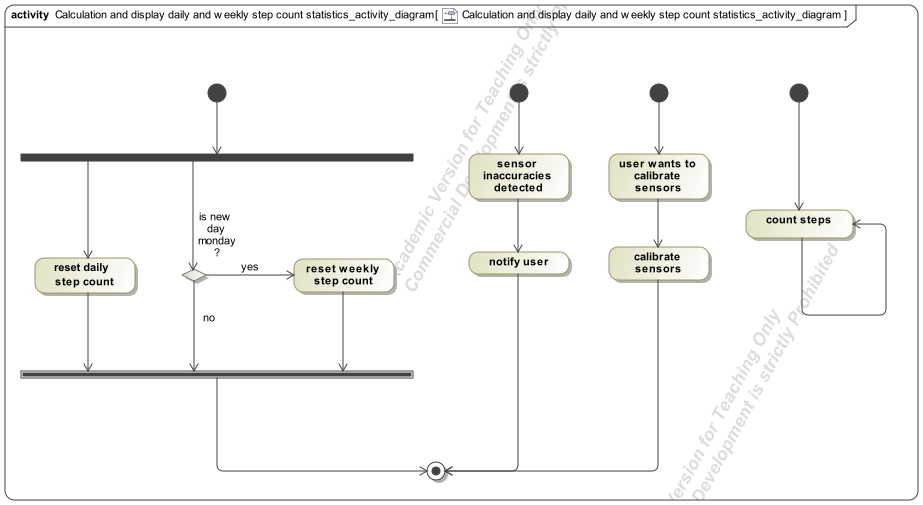
\includegraphics[width=\textwidth, angle=0]{Marc/req9/9activity.pdf}
		\end{figure}
		\newpage
		\begin{figure}[h!]
		    \centering
		    \captionsetup{labelformat=empty}
		    \caption{Your caption}
		    \includegraphics[width=\textwidth, angle=0]{Kreis2.pdf}
		\end{figure}
		\newpage

\section{Stefan Nguyen}
	\subsection{Requirement1}
		\begin{figure}[h!]
		    \centering
		    \captionsetup{labelformat=empty}
		    \caption{Your caption}
		    \includegraphics[width=\textwidth, angle=0]{Kreis2.pdf}
		\end{figure}
		\newpage
		\begin{figure}[h!]
		    \centering
		    \captionsetup{labelformat=empty}
		    \caption{Your caption}
		    \includegraphics[width=\textwidth, angle=0]{Kreis2.pdf}
		\end{figure}
		\newpage

\end{document}